\begin{frame}
\frametitle{About This Work...}

\emph{Managing Evolving Uncertainty in Trajectory Databases}~\cite{jeung2014managing}\\
H.~Jeung, H.~Lu, T.B.~Pedersen, S.~Sathe, M L.~Yiu.\\~\\

\begin{itemize}
  \item Published at \emph{TKDE' 2014}.
  \item A flexible trajectory modeling approach were proposed that takes into account model-inferred actual positions, time-varying uncertainty, and nondeterministic uncertainty ranges.
  \item Three estimators that effectively infer evolving densities of trajectory data were developed.
\end{itemize}

\end{frame}

%------------------------------------------------

\begin{frame}
\frametitle{Motivation}

\begin{itemize}
  \item \emph{Uncertainty management} is a central issue in trajectory databases
  \begin{fitemize}
    \item a common principle -- ``location uncertainty is captured by a certain range centered on the position recorded in the database''
  \end{fitemize}
  \item The old principle as the basis for the uncertain trajectory modelings is incapable of effectively capturing various types of uncertainty caused from different positioning sources
  \begin{fitemize}
    \item A location reported from a positioning system already bears some positional error, which implies that the exact location may not be identical to the reported position
    \item Positional errors may vary over time, as a result, the uncertainty should also change along time
    \item Bounding an area of uncertainty may cause loss of information
  \end{fitemize}
\end{itemize}

\end{frame}

%------------------------------------------------

\begin{frame}
\frametitle{Contributions}

\begin{itemize}

  \item \textbf{Evolving-density trajectory model}\quad to introduce a new uncertain trajectory model that represents a trajectory as time-dependent Gaussian distribution.

  \item \textbf{Evolving density estimators}\quad to propose three \emph{evolving density estimators} that infer time-varying densities of location data.

  \item \textbf{Efficient query processing}\quad to present an effective mechanism that indexes evolving density trajectories, and efficiently evaluates probabilistic range queries using the indexes.

\end{itemize}

\end{frame}

%------------------------------------------------

\begin{frame}
\frametitle{Existing Uncetain Trajectory Models}

There are two major reasons why uncertainty occurs in trajectory data:~\cite{pfoser1999capturing}
\begin{fitemize}
  \item one is known as \emph{measurement error} which is caused by limited accuracy of positioning technology, e.g., GPS error.
  \item the other is \emph{sampling error} that originates from discrete sampling of continuous movements of an object.
\end{fitemize}

Various \conceptbf{uncertainty models} have been proposed. These models commonly represent a trajectory using a sequence of uncertainty areas, so-called \emph{uncertain trajectory}.\\~\\

Each of the uncertainty areas captures the measurement and sampling errors.

\end{frame}

%------------------------------------------------

\begin{frame}
\frametitle{Existing Uncetain Trajectory Models}

\begin{figure}[tb]
  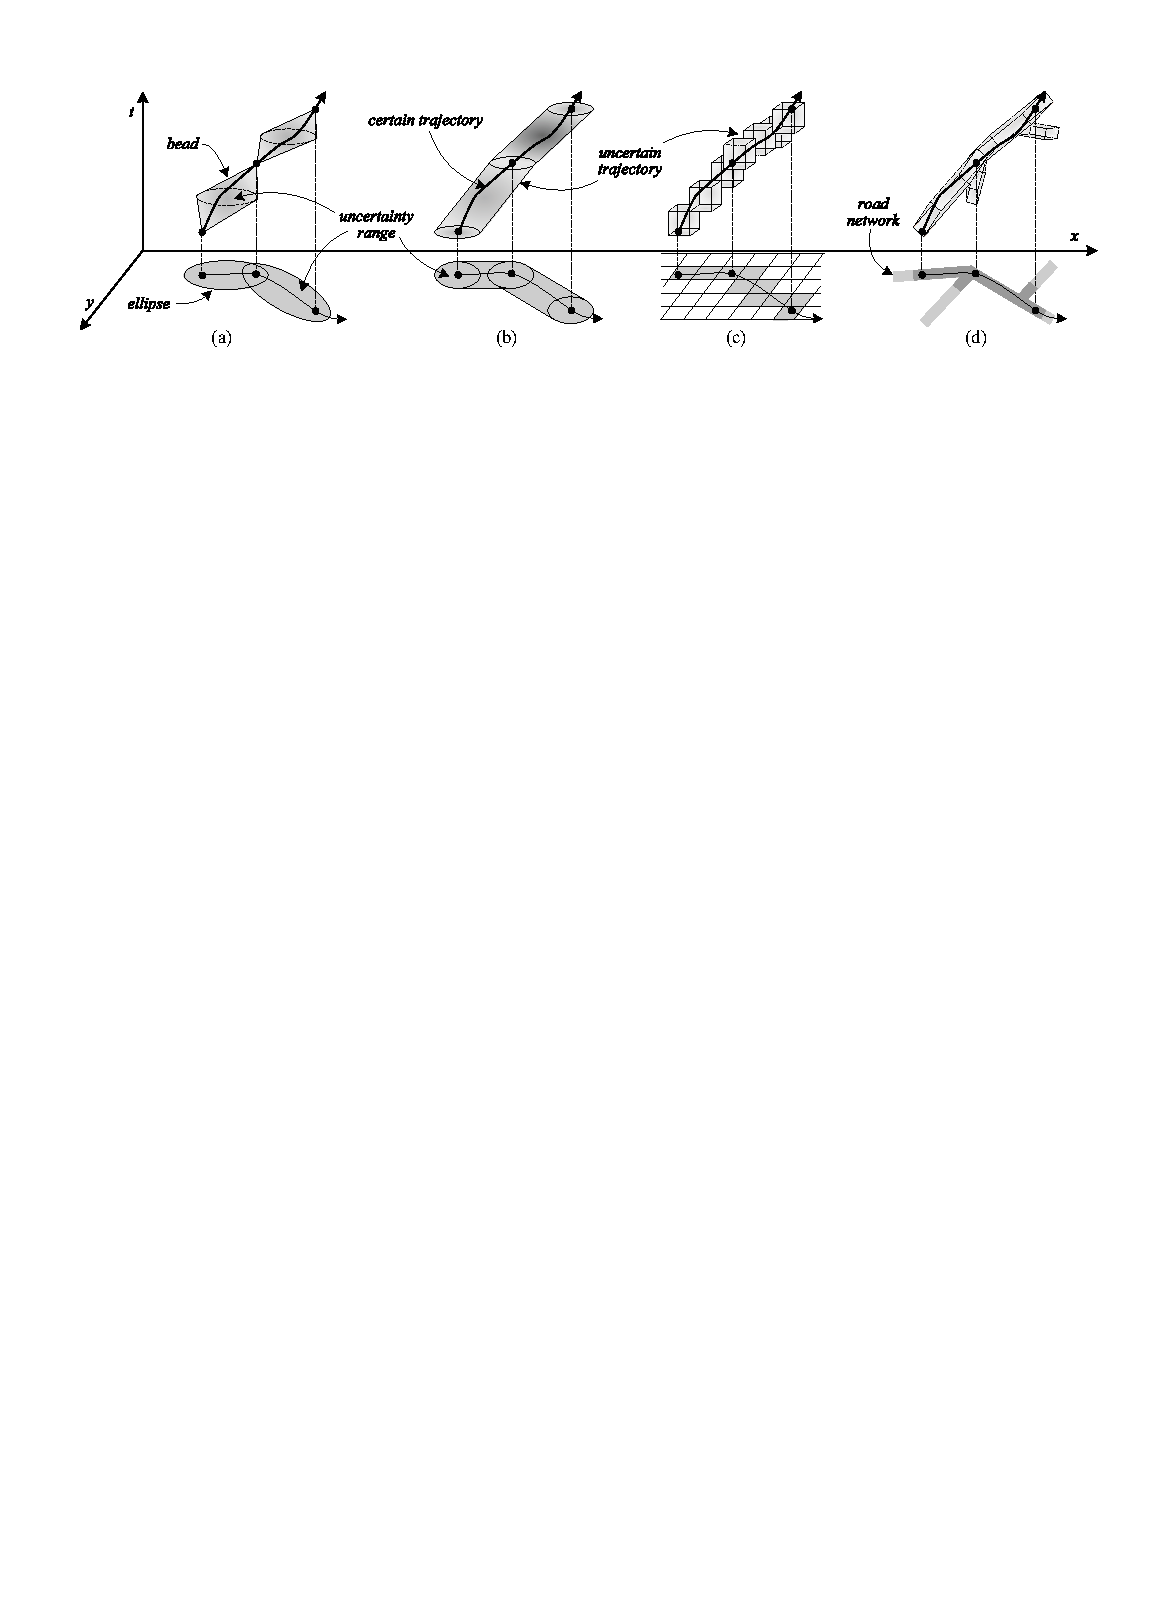
\includegraphics[width=\columnwidth]{figures/5-1/5-1-1.pdf}
\end{figure}

\vspace{10pt}

\footnotesize
\begin{tabular}{|l|c|c|c|c|}
\hline
\textbf{Models} & (a)Beads & (b)Cylinder & (c)Grid & (d)Network-constrained\\
\hline
\textbf{Works} & \cite{hornsby2002modeling,kuijpers2007trajectory} & \cite{frentzos2009effect,trajcevski2004managing,trajcevski2002geometry} & \cite{pelekis2009clustering,zhang2009effectively} & \cite{ding2008utr,ding2004uncertainty}\\
\hline
\end{tabular}

\end{frame}

%------------------------------------------------

\begin{frame}
\frametitle{Pitfalls of Existing Uncetain Trajectory Models}

\textrm{I.} \quad the uncertain trajectory models generally regard a location measured from positioning technology as a precise, actual location of an object, while modeling an uncertainty range based on the reported position as center.\\~\\

\textrm{II.} \quad some of the uncertain trajectory models assume that the degree of uncertainty is constant regardless of the cange of location or time.\\~\\

\textrm{III.} \quad the uncertain trajectory models bound the area of location uncertainty, typically using a circle with a user-specified radius. (\textit{it is inevitable to miss out some information when data processing is performed over any bounded uncertainty areas on unbounded distributions})

\end{frame}

%------------------------------------------------

\begin{frame}
\frametitle{Pitfalls of Existing Uncetain Trajectory Models}

\textrm{IV.} \quad most of the models assume that the probability density function (PDF) of a location is given, it is however a non-trival problem to compute the parameters of a PDF. \\~\\

\textrm{V.} \quad some models require additional data beyond location coordinates: the beads model uses maximum speed of object to determine the thickness of ellipse, while the network-constrained model needs map data encompassing the coverage of trajectories.

\end{frame}

%------------------------------------------------

\begin{frame}
\frametitle{Evolving-Density Trajectory: Key Principles}

\fsize{
\begin{table}
\begin{tabular}{|c|c|c|}
\hline
\textbf{Approaches} & \textbf{Applications} & \textbf{Works}\\
\hline
\emph{Kalman Filtering} & GPS data & \cite{lamarca2008location}\\
\hline
\emph{Particle Filtering} & mobile RFID readings & \cite{tran2009probabilistic}\\
\hline
\emph{Map Matching} & network-constrained objects' locations & \cite{brakatsoulas2005map}\\
\hline
\emph{Sensor Fusion} &  & \cite{bessho2009location}\\
\hline
\end{tabular}
\caption{Approaches for processing noise-contaminated raw location data}
\end{table}
}

\begin{block}{Actual Position}
  Above approaches provide means that can infer more reliable positions where an object was actually located. The evolving-density trajectory model supports such an inferred location as an actual location of the object, which serves as the center point of an uncertainty range.
\end{block}

\end{frame}

%------------------------------------------------

\begin{frame}
\frametitle{Evolving-Density Trajectory: Key Principles}

\begin{block}{Gaussian Distribution}
  Measurement errors in positioning typically obey Gaussian distributions. The approach models that an object's location follows Gaussian distributions.
\end{block}

\begin{columns}

  \column{0.5\textwidth}
  \begin{figure}[tb]
    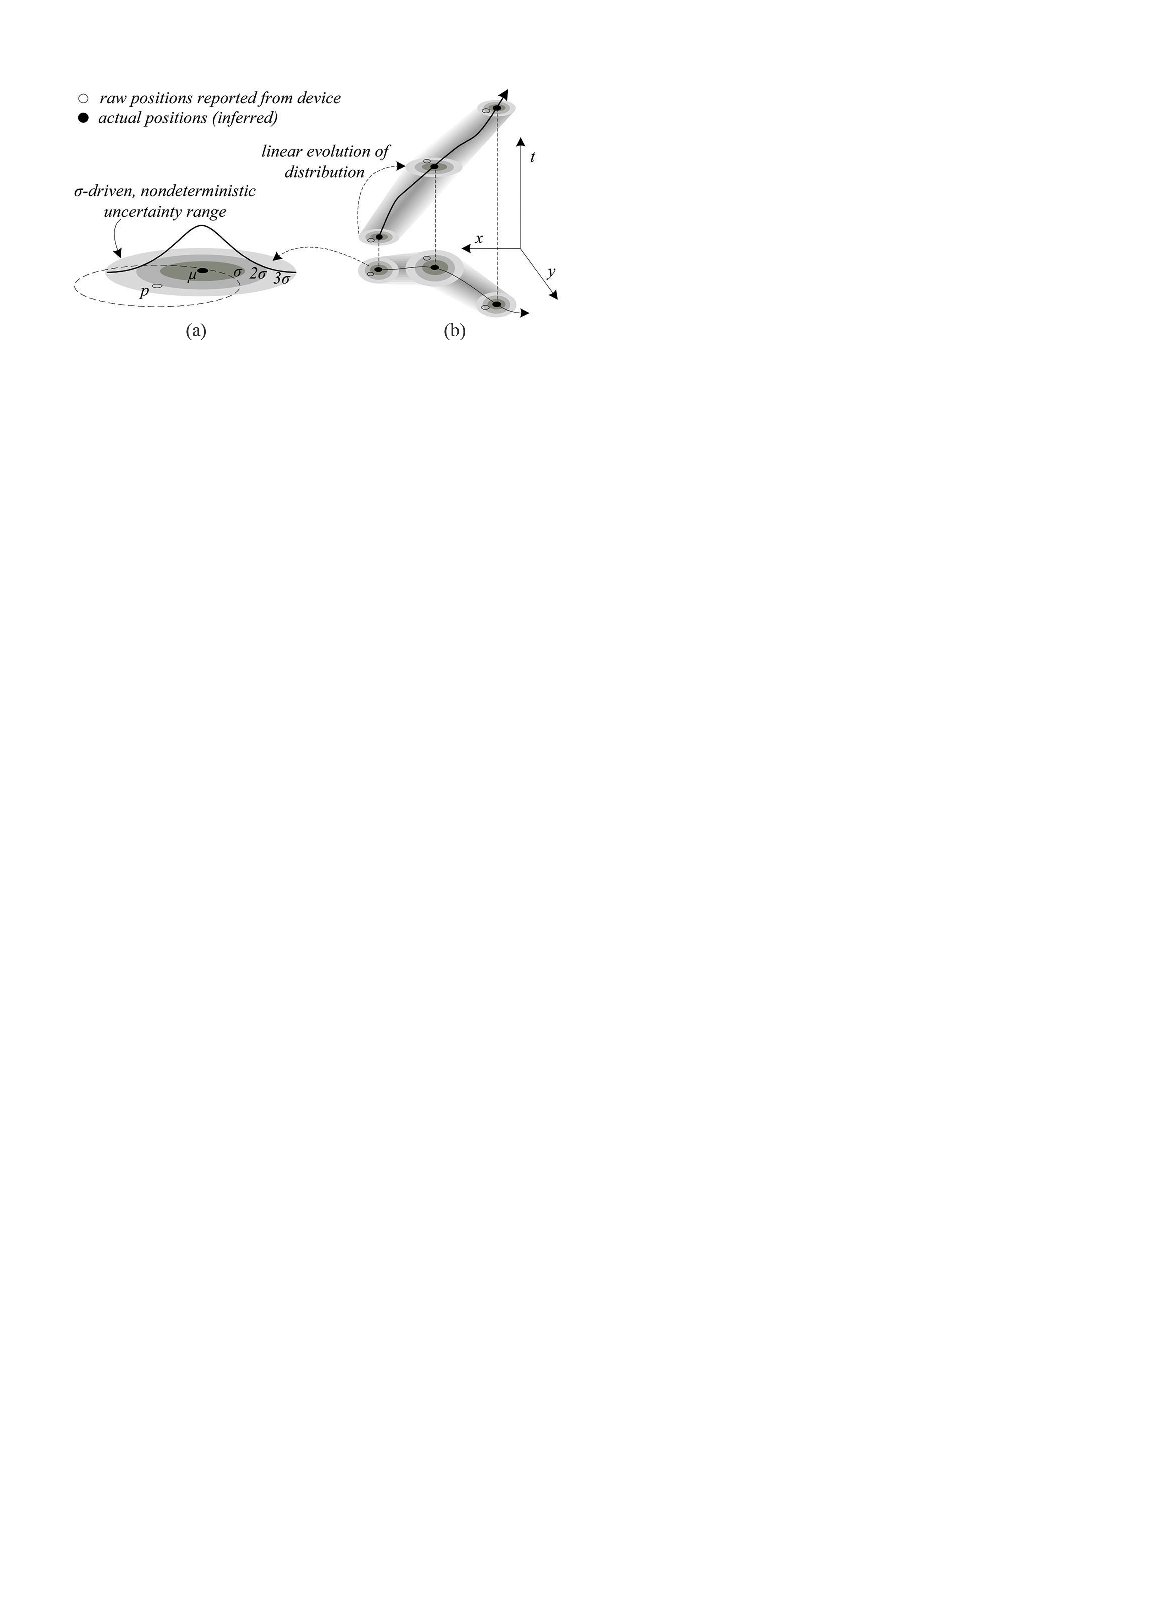
\includegraphics[width=\columnwidth]{figures/5-1/5-1-2.pdf}
  \end{figure}

  \column{0.5\textwidth}
  \begin{example}
    \fsize{
      The uncertain position models the object's acutal location as the mean $\mu$, corresponding to the raw position $p$. In addition, the standard deviation $\sigma$ reflects the degree of uncertainty with respect to $\mu$.
    }
  \end{example}

\end{columns}

\end{frame}

%------------------------------------------------

\begin{frame}
\frametitle{Evolving-Density Trajectory: Key Principles}

\begin{block}{$\sigma$-Driven, Nondeterministic Uncertainty Range}
  Do not represent an uncertainty range in a deterministic manner. Instead, keep only the information of deviation $\sigma$, and then dynamically compute the minimum bound for each data point (distribution) that can satisfy a given query condition.
\end{block}

\end{frame}

%------------------------------------------------

\begin{frame}
\frametitle{Evolving-Density Trajectory: Key Principles}

\begin{block}{Time-Dependent Uncertainty}
  To reflect the time-varying errors caused from positioning systems, it models each uncertain position in an evolving-density trajectory differs from another, meaning that each uncertain position has different values for $\mu$ and $\sigma$.
\end{block}

\end{frame}

%------------------------------------------------

\begin{frame}
\frametitle{Evolving-Density Trajectory: Key Principles}

\begin{block}{Linear Evolution of Distribution}
  In-between two consecutive uncertain positions, it assumes that the distributions of actual positions evolve linearly. Consider an object's movements between two positions are commonly modeled as linear in certain trajectories, moreover, it is
\end{block}

\end{frame}

%------------------------------------------------

\begin{frame}
\frametitle{Framework Overview}

\begin{columns}

  \column{0.5\textwidth}
  \begin{figure}[tb]
    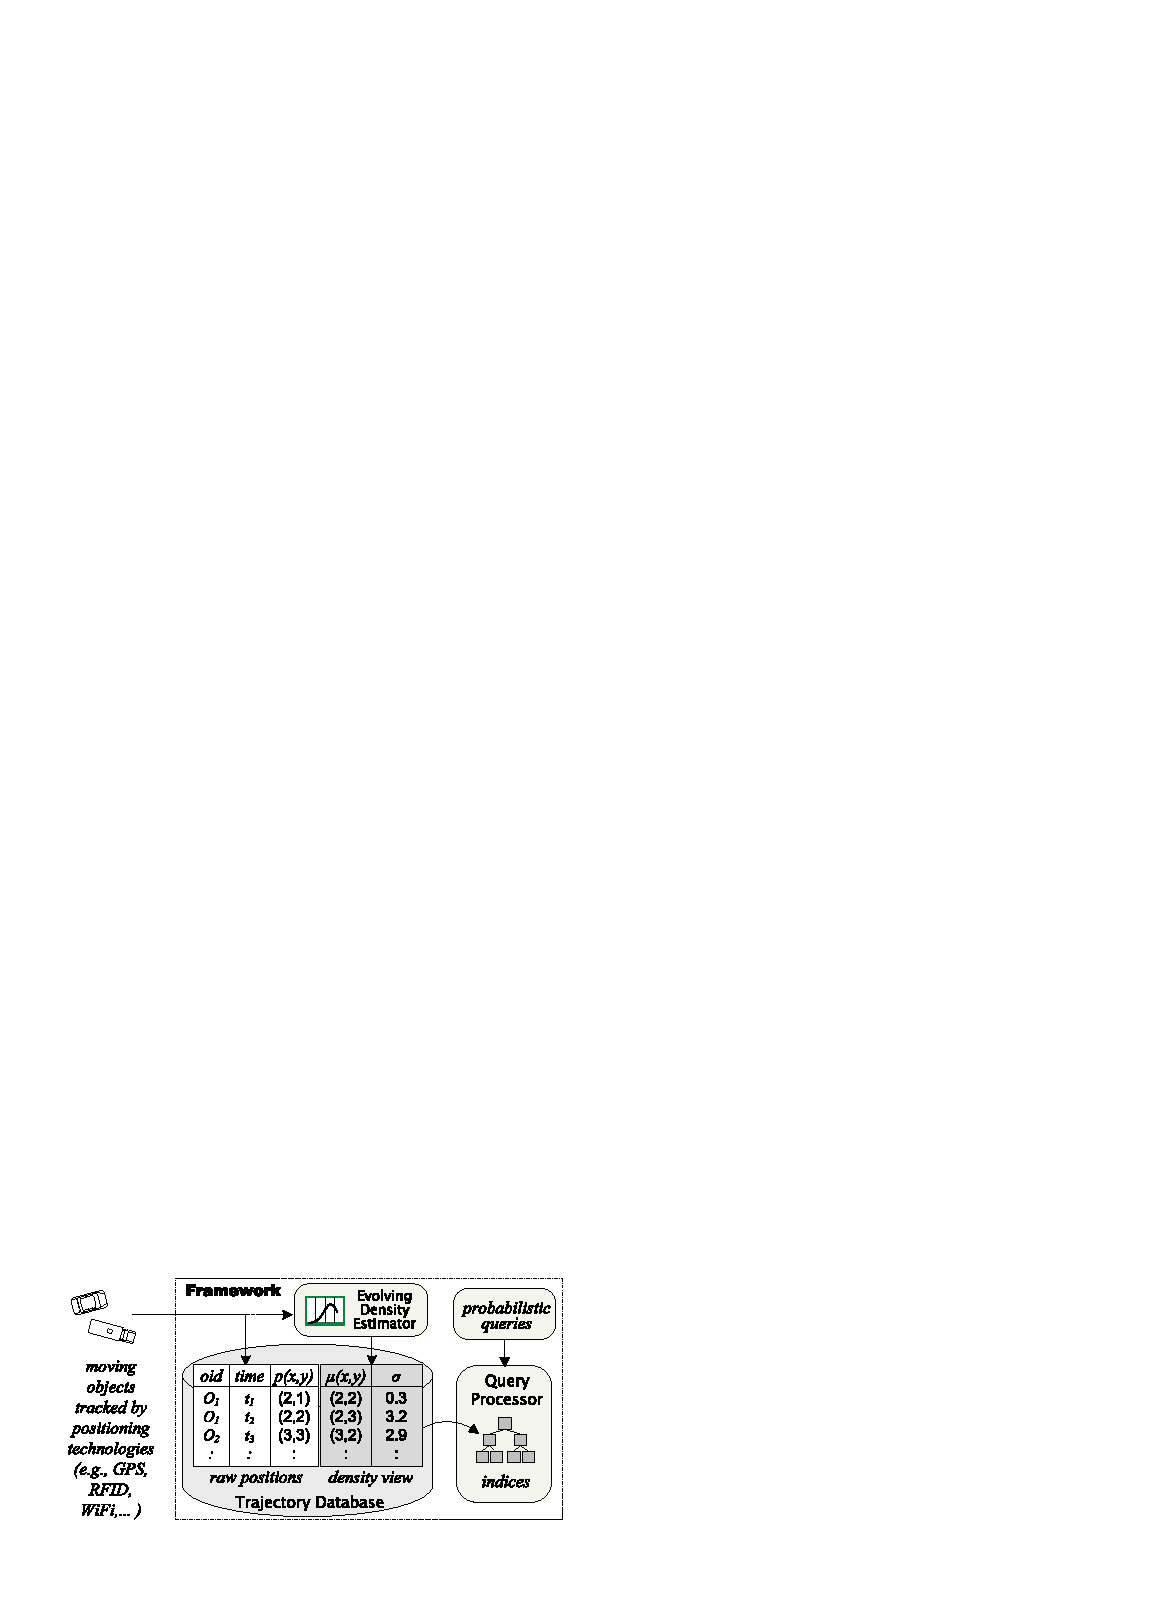
\includegraphics[width=\columnwidth]{figures/5-1/5-1-3.pdf}
  \end{figure}

  \column{0.5\textwidth}
  \ssize{
  \conceptbf{Evolving Density Estimator}\quad computes the probability distribution of an object's position at each time. The component takes a certain number of recent positions in a trajectory, and infers a Gaussian distribution at a current time. Domian-specific knowledge is supported for user-given estimator.
  }
\end{columns}

\vspace{25pt}

\begin{columns}

  \column{0.5\textwidth}
  \ssize{
  \conceptbf{Trajectory Database}\quad manages not only the raw positions, but also the correponding probablity distributions derived from an evolving density estimator.
  }

  \column{0.5\textwidth}
  \ssize{
  \conceptbf{Query Processor}\quad supports efficient processing of probabilistic range queries on the evolving-density trajectories managed in the system.
  }

\end{columns}

\end{frame}

%------------------------------------------------

\begin{frame}
\frametitle{Evolving Density Estimator}

\fsize{

Generalized AutoRegressive Conditional Heteroskedasticity - \conceptbf{GARCH} model~\cite{shumway2010time} is a well-established stochastic volatility model that is generally used to assess an investment risk in finance, since volatility represents the degree of deviation from what the data is supposed to be, reflecting a measure of risk for investing.\\~\\

The implemented estimators have extended the GARCH model to handle multi-dimensional location data since the model can assess the deviation of a raw position from where the corresponding actual position is supposed to reside on.\\~\\

The estimators employ a sliding window that takes a $H$ number of consecutive positions for the estimation, and then repeat the same estimation process using the next $H$ positions.\\~\\

Given a sliding window of positions $S^{H}_{t-1} \in \mathbb{R}^{H \times 2}$, the estimators infer two quantities: 1) the expected true position $\hat{p_t} = (\hat{x_t}, \hat{y_t})$ at time $t$; 2) a standard deviation $\hat{\sigma_t}$.

}

\end{frame}

%------------------------------------------------

\begin{frame}
\frametitle{Conditional Correlation Estimator}

\conceptbf{Conditional Correlation Estimator ($C^2$-Est)} uses a multivariate mean inference model for estimating the expected true position $\hat{p_t} = (\hat{x_t}, \hat{y_t})$, where $\hat{x_t}$ and $\hat{y_t}$ are the $x$- and $y$-coordinate, respectively.\\~\\

VAR (\underline{V}ector \underline{A}uto\underline{R}egressive) Model can exploit the interdependencies of $\hat{x_t}$ and $\hat{y_t}$ for inferring the actual position $\hat{p_t}$.

\begin{equation}
  \hat{p_t} = \phi_0 + \sum_{j=1}^{k}\phi_j p_{t-j}
\end{equation}

where $\phi_1,...,\phi_k$ are autoregressive coefficients of each size $2 \times 2$, $\phi_0$ is a $2$-dimensional vector, and $t > k$.~\cite{shumway2010time}

\end{frame}

%------------------------------------------------

\begin{frame}
\frametitle{Conditional Correlation Estimator}

For inferring the deviation $\hat{\sigma_t}$, $C^2$-Est uses the constant conditional correlation (CCC) model~\cite{bauwens2006multivariate}. \\~\\

The 2-by-2 conditional variance matrix of $p_i$, denoted as $\Lambda_i$, is defined as:

\begin{equation}
  \Lambda_i = Var(p_i - \hat{p_i} | F_{i-1}), \Lambda_i = Var(a_i | F_{i-1})
  \label{equation:variance_matrix}
\end{equation}

where $Var(a_i | F_{i-1})$ is the variance matrix of $a_i$, given all the information $F_{i-1}$ available until time $i-1$.

\end{frame}

%------------------------------------------------

\begin{frame}
\frametitle{Conditional Correlation Estimator}

The CCC model uses the errors $a_i$ from the VAR($k$) model to represent the conditional variance matrix $\Lambda_i$ in Equation.~(\ref{equation:variance_matrix}).

\begin{equation}
  a_i = \Lambda_i^{1/2}, \Lambda_{nm,i} = \rho_{nm} \sqrt{\lambda_{nn,i}\lambda_{mm,i}}
\end{equation}

where $\Lambda_{nm,i}$ is the value on row $n$ and column $m$ of matrix $\lambda_{i}$, $\lambda_{nn,i}$ and $\lambda_{mm,i}$ are defined using an univariate GARCH(1,1) model, $\rho_{nm}$ are the constant conditional correlations with $\rho_{nn} =1$.\\~\\

Given $\rho_{nm}$ and the univariate GARCH(1,1) models for $\lambda_{nn,i}$ and $\lambda_{mm,i}$, $C^2$-Est first infers $\lambda_{nn,t}$ and $\lambda_{mm,t}$ using the univariate GARCH models.

\begin{equation}
  \hat{\Lambda_t} = (\rho_{nm} \sqrt{\lambda_{nn,t} \lambda_{mm,t}})
\end{equation}

\end{frame}

%------------------------------------------------

\begin{frame}
\frametitle{Radial Estimator}

\conceptbf{Radial Estimator (R-Est)} also uses VAR model for inferring the expected true position $\hat{p_t}$. Differently, it employs a more efficient model, i.e., Radial GARCH model, for inferring $\sigma_t$.\\~\\

Specifically, the R-Est estimator starts by computing the Euclidean norms of the errors $a_i$ by the VAR($k$) model, denoted at $\gamma_i$.\\~\\

$a_i$ are the possible varations, such that positions $p_i$ are derived from the expected true positions $\hat{p_i}$. This means that $\gamma_i$ for each $i$ gives the uncertainty. Thus, R-Est uses $\gamma_i$ for inferring the deviation $\hat{\sigma_t}$.

\end{frame}

%------------------------------------------------

\begin{frame}
\frametitle{AutoRegressive Radial Estimator}

\conceptbf{AutoRegressive Radial Estimator (AR-Est)} is a variant of R-Est. For inferring the deviation $\hat{\sigma_t}$, this new estimator takes the same RGARCH model used in R-Est.\\~\\

AR-Est takes a different approach for the inference of an actual position. It decomposes the multivariate inference into two separate one-dimensional inferences, it uses univariate AR models for inferring $\hat{x_t}$ and $\hat{y_t}$ separately.\\~\\

Given a sliding window $S^{H}_{t-1}$, the AR($l$) model models $x_i = \hat{x_i} + a_{x,i}$, where $t-H \leq i \leq t-1$. Given an AR($l$) model, it infers the expected true position $\hat{x_t}$ as:~\cite{shumway2010time}

\begin{equation}
  \hat{x_t} = \phi_{x0} + \sum_{j=1}^{l}\phi_{xj}p_{t-j}
\end{equation}

\end{frame}
